\section{Задание}

\subsection{Постановка задачи}

Граф, вариант 15.\\

Для чтения и обработки графа из файла, был добавлен следующий код (Листинги \ref{lst:lst1} и \ref{lst:lst2})

\subsection{Дополнение к коду}
\captionsetup{singlelinecheck = false, justification=raggedright}
\lstinputlisting[label=lst:lst1, caption=Загрузка данных, language=c++, firstline=263, lastline=311]{./inc/read.cpp}
\newpage
\lstinputlisting[label=lst:lst2, caption=Обработка данных, language=c++, firstline=31, lastline=41]{./inc/read.cpp}

Сам граф представлен на рисунке~\ref{fig:graph}

\begin{figure}[H]
    \centering
    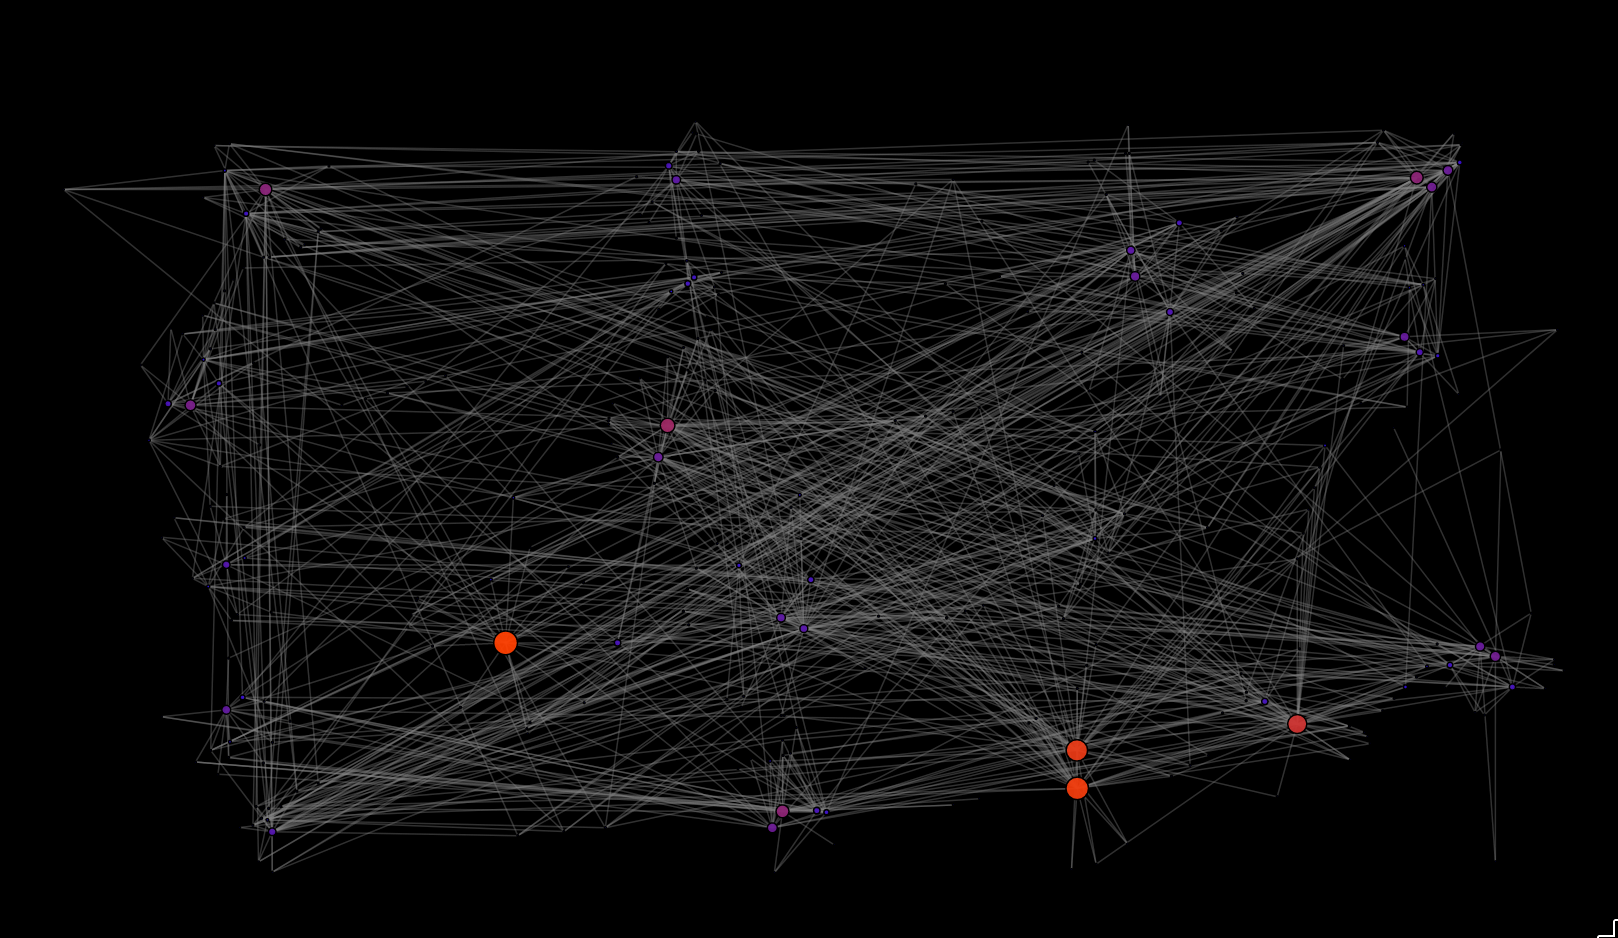
\includegraphics[scale=0.5,width=\textwidth]{inc/img/graph}
    \caption{Граф, вариант 15.}
    \label{fig:graph}
\end{figure}

